% SCH4U Date: ___________________________________________

% Lab: Density of Rubber Stoppers

% Purpose:
% ● To determine the density of two sizes of rubber stoppers
% ● To write up a complete lab report using proper format
% Materials:
% ● graduated cylinder (any size)
% ● two rubber stoppers (small & large)
% ● beaker (any size)
% ● mass scale
% ● dropper (if necessary)
% Procedure:
% Part 1: Density of Small Rubber Stopper:
% a. Take the mass of the small rubber stopper using the electronic balance.
% b. Fill a graduated cylinder about half-way with water. Record the initial water level.
% c. Drop the rubber stopper into the water. Avoid trapping air bubbles in the water. Stir the water to remove the bubbles if
% necessary. Record the new water level.
% d. Calculate the density of the small rubber stopper.
% Part 2: Density of Large Rubber Stopper:
% a. Devise a method to determine the density of the large rubber stopper using a similar procedure as Part I. You cannot
% request a larger graduated cylinder. ☺
% b. Write out a detailed procedure flowchart to perform in the laboratory. Include the exact amounts of materials & every
% piece of equipment that will be used. It should be detailed enough so that a complete stranger can understand & be
% able to conduct all steps of your procedure without your presence needed.
% Observations Table:
% ● Design your own observations table. Be sure to leave enough space to record masses & volumes. Any additional
% observations are welcome. Record all observations in pen. Get your observations initialed by your teacher before you
% leave class. You will need to submit this signed form with your completed lab report.

% Prelab Instructions:
% Have the following completed on a sheet of
% paper before the lab date:
% ● Date, Title & Purpose
% ● Introduction
% ● Procedure flowchart (for Part 2 only)
% ● Observations Table(s) drawn & ready to
% use

% Postlab Instructions:
% In addition to the prelab, the completed lab report will have
% the following: (to be completed in class)
% ● Lab partner’s name(s)
% ● Completed observation(s) table(s)
% ● Discussion Questions (to be announced on day of lab)
% ● Conclusion

% Important Notes:
% 1. You will be working individually throughout this task (most labs you would be allowed to work with a partner for the
% experimental component)
% 2. Do not be overly concerned about getting the “right” answer...the focus of this lab (& every lab thereafter) is honest
% reporting of results & clarity of written work
% 3. It is okay to make mistakes...when recording observations & you make a mistake, simply cross out the error using a
% single line.

% METHOD/PROCEDURE
% • consists of a flowchart showing how to do the lab (sentence fragments are acceptable)
% • a long vertical arrow (or series of arrows), drawn with a ruler, represents the order of events
% • substances added are shown by a labeled arrow flowing into the main arrow from the side
% • anything done to the experimental mixture is labeled beside the main arrow in a location appropriate to the time at which
% it is done (see example below)
% • if components of the mixture are separated &/or treated differently, branches must split off the main arrow in the
% appropriate spot

% Materials/Equipment Actions Taken

% OBSERVATIONS
% • observations can be qualitative or quantitative (or both!) & are based only on what is seen or measured
% • table format (see below) must be used if substances are being compared
% • observations must follow the order of the procedure
% • all qualitative observations must be in table form as a series of point-form statements
% • all raw quantitative observations (every measurement) must be organized into a table
% • all tables must have a border, & lines separating columns & rows
% • each table must have a number & a descriptive title (i.e., Table 1: Observations of Esters)
% • rows & columns must be used logically & appropriately to organize the data
% Table 1: Measurements of Length & Width
% Object Length (m) Width (m)

% • any calculation using the raw data goes under the Results/Analysis section, & must be organized into a summary table,
% along with a sample calculation provided below the table
% • include rough observations recorded during the lab into your lab report, attached to the end of the lab report
% as an Appendix
% RESULTS/ANALYSIS
% • can be quantitative (calculations) or qualitative (an explanation for the observations witnessed)
% • if quantitative:
% • correct problem-solving format & significant digits are required
% • a heading must be used to indicate what is being determined
% • if a calculation is repeated multiple times, show one sample calculation for each type of calculation & give the
% answers for the rest in a table
% • may include balanced chemical equations &/or graphs
% • correct graphing format must be used
% • graphs may be completed on a computer & included in the lab report
% • every graph must have a number & descriptive title (i.e., Figure 1: Concentration of Iodine Solution)
% • provide a brief explanation for the graph
% • any questions in this section should be answered separately & in order, & the questions themselves should NOT be
% copied from the lab sheet
% DISCUSSION
% • consists of answers to lab questions
% • should be answered separately & numbered, in order
% • written in complete, correct sentences which clearly indicate what the question was (do not include the questions
% in the lab report)
% • do not require research to answer unless explicitly stated
% • must include reference to appropriate results where required
% • state table or figure number & data or observation that supports the answer to the question
% • usually requires thorough analysis of the data presented in the Results section
% • avoid “human error” in error analysis & focus on the fundamental assumptions made in the lab
% Added 10.0 mL of water

% 100 mL beaker

% Added 1.00 g salt
% Stirred contents in beaker

% Stirring Rod

% 10

% • if asked for more than one idea, use one paragraph per idea...for example, if asked for 3 significant sources of error,
% use one paragraph for each source of error
% • remember to identify the error, then explain the error, & then determine how this error affected the final objective
% of the lab

% CONCLUSION
% • consists of one or two sentences
% • should make specific reference to the significant result that addresses the purpose
% • if the lab is quantitative, state the final numerical results of the lab
% • if the lab is qualitative, state describe the results of the lab
% Summary/Last Additional Notes Regarding Lab Reporting:
% • lab reports are due at the beginning of class...if necessary, print BEFORE coming to class...do not use class time to
% do your printing!
% • lab partner(s) names go near the top of the first page of the lab report
% • the date on a lab report is the date the lab was performed
% • use passive tense throughout a lab report
% • the words “one” & “they” can refer to objects or people...if referring to people, it becomes a personal pronoun & is
% no longer passive tense
% • use past tense from the Observations section & onwards
% • every unique idea must have its own paragraph
% • procedure flowcharts, tables & calculations should appear in its entirety on a page (do not split them across different
% pages, unless it is unavoidable)
% • keep all rough notes taken during a lab & include it as an Appendix, at the end of the lab report
% • when answering questions, do not assume the reader can read your mind...explain everything clearly but at the same
% time, be concise & precise!

\documentclass{article}
\usepackage[margin=1in]{geometry}
\usepackage{tikz}

% Macros for procedure flowchart auto-spacing
\newcommand{\stepy}{0}
\newcommand{\spacing}{0.75}
\newcommand{\lstep}[1]{%
    \pgfmathsetmacro{\newy}{\stepy - \spacing}%
    \xdef\stepy{\newy}%
    \draw[<-] (0, \stepy) -- (-1.5, \stepy) node[left] {#1};%
}
\newcommand{\rstep}[1]{%
    \pgfmathsetmacro{\newy}{\stepy - \spacing}%
    \xdef\stepy{\newy}%
    \draw[<-] (0, \stepy) -- (1.5, \stepy) node[right] {#1};%
}

\begin{document}
\title{Lab 0 - Rubber Stoppers}
\author{Aaron Huang}
\date{\today}
\maketitle
\section{Purpose}
The purpose of this lab is to determine the density of two sizes of rubber stoppers and to write up a complete lab report using proper format.
\section{Materials}
\begin{itemize}
    \item graduated cylinder (200 mL)
    \item two rubber stoppers (small \& large)
    \item beaker (50 mL)
    \item beaker (250 mL)
    \item water
    \item mass scale
    \item dropper
\end{itemize}
\section{Procedure}
% part 1
\subsection{Part 1: Density of Small Rubber Stopper}
\begin{center}
    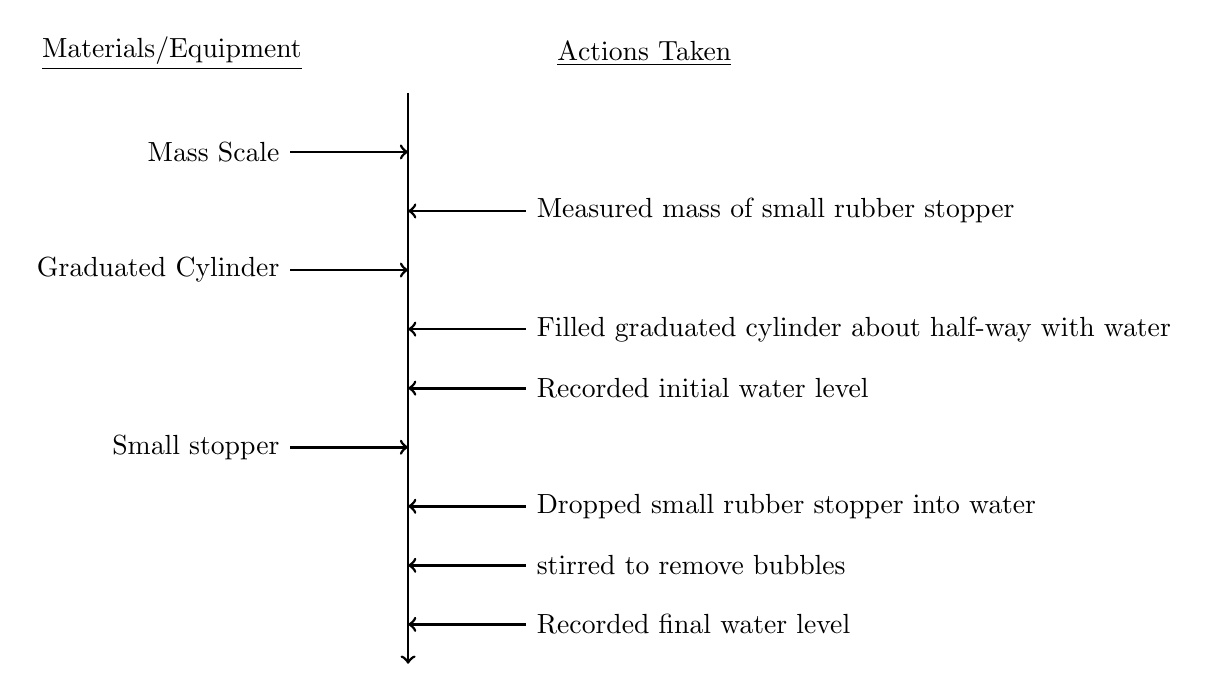
\begin{tikzpicture}[line width=1pt]

        % Reset/Initialize y-offset for the flowchart
        \renewcommand{\stepy}{0}

        % Column Headers
        \node at (-3, 0.5) {\underline{Materials/Equipment}};
        \node at (3, 0.5) {\underline{Actions Taken}};

        % --- Step 1: Mass of Small Rubber Stopper ---
        \lstep{Mass Scale}
        \rstep{Measured mass of small rubber stopper}

        % --- Step 2: Initial Water Level ---
        \lstep{Graduated Cylinder} 
        \rstep{Filled graduated cylinder about half-way with water}
        \rstep{Recorded initial water level}

        % --- Step 3: Final Water Level ---
        \lstep{Small stopper}
        \rstep{Dropped small rubber stopper into water}
        \rstep{stirred to remove bubbles}
        \rstep{Recorded final water level}

        % Main vertical arrow (Dynamic length based on final \stepy)
        \draw[->] (0, 0) -- (0, \stepy - 0.5);

    \end{tikzpicture}
\end{center}

\subsection{Part 2: Density of Large Rubber Stopper}

\begin{center}
    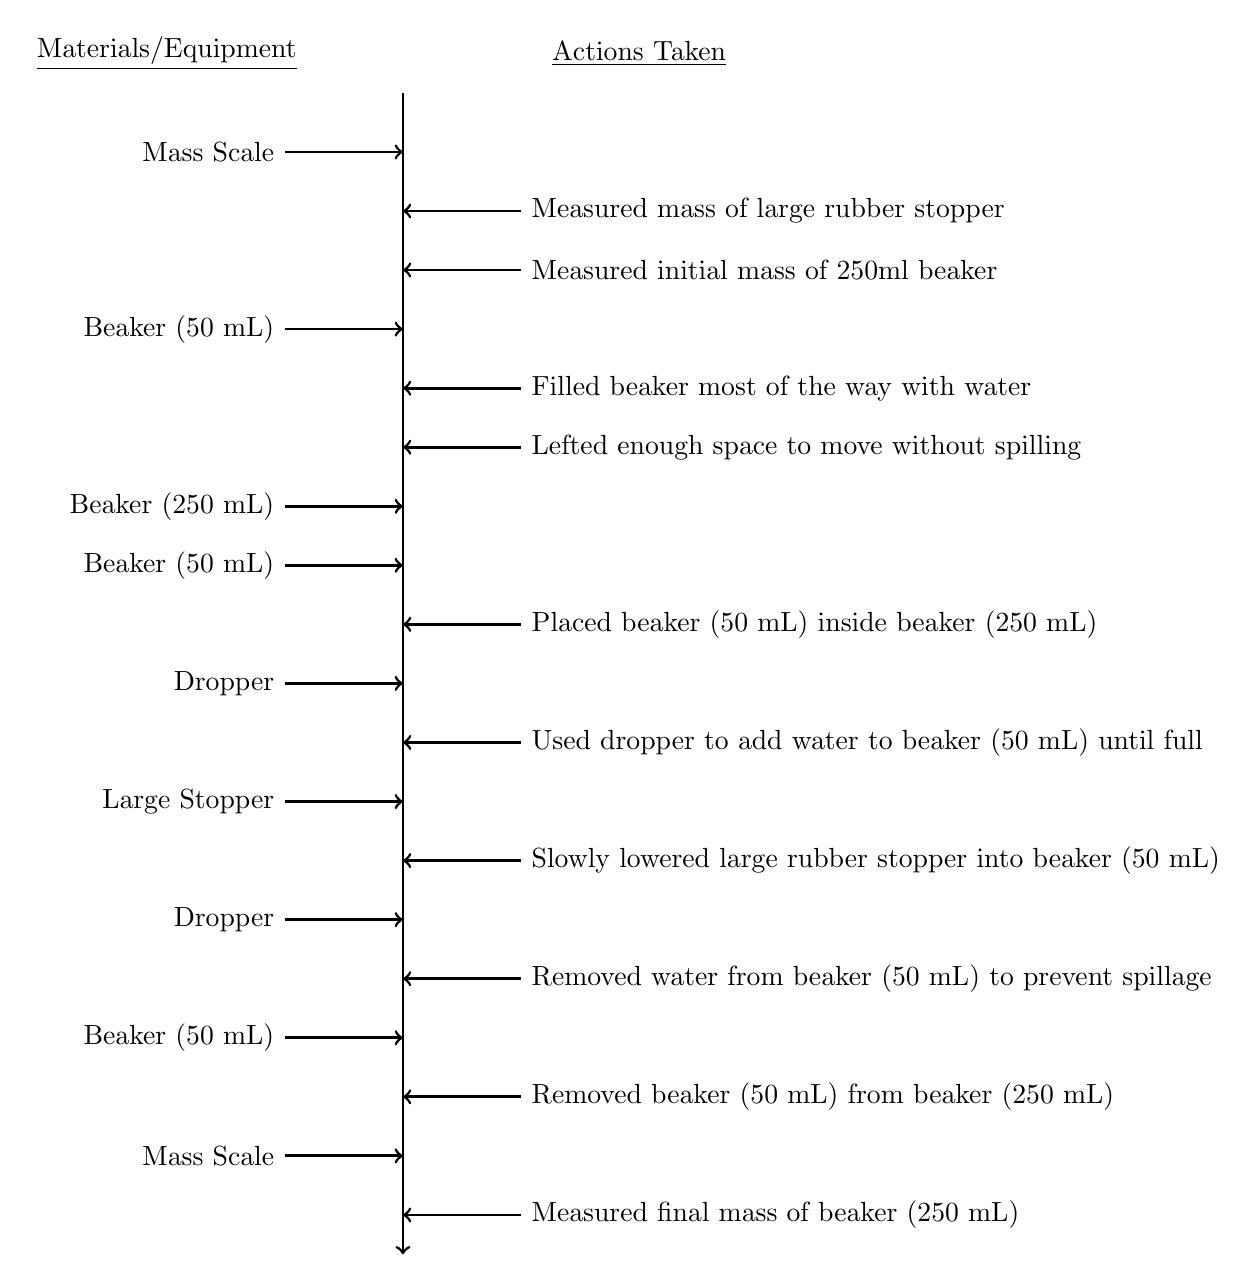
\begin{tikzpicture}[line width=1pt]
        % Reset/Initialize y-offset for the flowchart
        \renewcommand{\stepy}{0}

        % Column Headers
        \node at (-3, 0.5) {\underline{Materials/Equipment}};
        \node at (3, 0.5) {\underline{Actions Taken}};

        % --- Step 1: Mass of Large Rubber Stopper ---
        \lstep{Mass Scale}
        \rstep{Measured mass of large rubber stopper}
        \rstep{Measured initial mass of 250ml beaker}

        % --- Step 2: Initial Water Level in Beaker ---
        \lstep{Beaker (50 mL)}
        \rstep{Filled beaker most of the way with water}
        \rstep{Lefted enough space to move without spilling}
        \lstep{Beaker (250 mL)}
        \lstep{Beaker (50 mL)}
        \rstep{Placed beaker (50 mL) inside beaker (250 mL)}
        \lstep{Dropper}
        \rstep{Used dropper to add water to beaker (50 mL) until full}
        \lstep{Large Stopper}
        \rstep{Slowly lowered large rubber stopper into beaker (50 mL)}
        \lstep{Dropper}
        \rstep{Removed water from beaker (50 mL) to prevent spillage}
        \lstep{Beaker (50 mL)}
        \rstep{Removed beaker (50 mL) from beaker (250 mL)}
        \lstep{Mass Scale}
        \rstep{Measured final mass of beaker (250 mL)}
        
        % Main vertical arrow (Dynamic length based on final \stepy)
        \draw[->] (0, 0) -- (0, \stepy - 0.5);
        
    \end{tikzpicture}
\end{center}

\section{Observations}
\begin{table}[h!]
    \centering
    \caption{Observations of Rubber Stoppers}
    \label{tab:observations}
    \vspace{0.125 in}
    \begin{tabular}{|c|c|c|c|}
        \hline
        \textbf{Rubber Stopper Size} & \textbf{Mass (g)} & \textbf{Initial Measurement} & \textbf{Final Measurement} \\
        \hline
        Small &  &  &  \\
        \hline
        Large &  &  &  \\
        \hline
    \end{tabular}

\end{table}



\end{document}